\chapter{不等式}

本章讨论不等式。不等式常用于讨论函数最大值最小值,在工程实践中也有现实意义。

本章要点:
\begin{itemize}
    \item 不等式的性质。
    \item 四类均值及其不等式。
    \item 基本不等式和二次函数。
\end{itemize}

\newpage
\section{等式性质与不等式性质}

本节要点:
\begin{itemize}
    \item 熟练掌握等式的性质;
    \item 熟练掌握不等式的性质。
\end{itemize}

~

若$a,b,c\in \mathbb{R} $,则有等式的性质:
\begin{itemize}
    \item 性质1:$a=b\Rightarrow b=a$;
    \item 性质2:$a=b,b=c\Rightarrow a=c$;
    \item 性质3:$a=b\Rightarrow a\pm c=b\pm c$;
    \item 性质4:$a=b\Rightarrow ac=bc$;
    \item 性质5:$a=b,c\ne 0\Rightarrow a/c=b/c$。
\end{itemize}

\begin{tcolorbox}
性质1表示了对等性,性质2表示了传递性,性质3表示了加减不变性,性质4、5表示了乘除的不变性。
\end{tcolorbox}

根据算术运算的法则,不难得出不等式的性质,若$a,b,c\in \mathbb{R} $,则有不等式的性质:
\begin{itemize}
    \item 性质1:$a>b\Leftrightarrow b<a$;
    \item 性质2:$a>b,b>c\Rightarrow a>c$;
    \item 性质3:$a>b\Rightarrow a\pm c>b\pm c$;
    \item 性质4:$a>b,c>0\Rightarrow ac>bc$,$a>b,c<0\Rightarrow ac<bc$;
    \item 性质5:$a>b,c>d\Rightarrow a+c>b+d$;
    \item 性质6:$a>b>0,c>d>0\Rightarrow ac>bd$;
    \item 性质7:$a>b>0\Rightarrow a^n>b^n,n\in \mathbb{N} \text{且}n>0$。
\end{itemize}

~

等式和不等式的性质本身并无难度,关键掌握两个点。

首先,不等式在代数中表示一个约束,通常多个约束是逻辑与的关系,除非特别指明逻辑或,所以如下的三种表示方法是等价的:
\begin{align*}
&A<B,A>C \\
&C<A<B \\
&\left\{ \begin{array}{c}
	A<B\\
	A>C\\
\end{array} \right.
\end{align*}

其次,在判断两个式子的不等关系时,常用的方法是相减后和0比大小。当然也可以相除后和$\pm 1$比大小,但高中阶段不常用。

~

\begin{example}[拓广探索12,难度:$\star \star \star \star $]
火车站有某公司待运的甲种货物1530t,乙种货物1150t,现计划用A、B两种型号的货厢共50节运送这批货物。已知35t甲种货物和15t乙种货物可装满一节A型货厢,25t甲种货物和35t乙种货物可装满一节B型货厢,据此安排A、B两种货厢的节数,共有几种方案?若每节A型货厢的运费是0.5万元,每节B型货厢的运费是0.8万元,哪种方案的运费较少?
\end{example}

解:

设两种型号货厢各$A,B$个,不难得到如下4个约束:
\begin{itemize}
    \item 共运载甲种货物不少于1530t,$35A+25B\geqslant 1530$;
    \item 共运载乙种货物不少于1150t,$15A+35B\geqslant 1150$;
    \item 两种货厢共不多于50节,$A+B\leqslant 50$;
    \item 货厢为自然数,$A,B\in \mathbb{N} $。
\end{itemize}
取$A$为横坐标,$B$为从坐标,图形如下:
\begin{figure}[h]
\centering
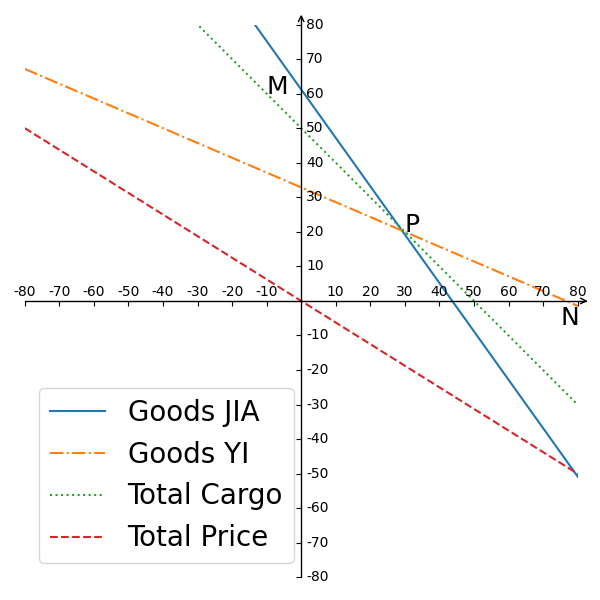
\includegraphics[height=8cm]{2.1-1.png}
\end{figure}

反映到图象上,即要求:
\begin{itemize}
    \item 共运载甲种货物不少于1530t,在蓝实线的上方;
    \item 共运载乙种货物不少于1150t,在橙点划线的上方;
    \item 两种货厢共不多于50节,在绿虚线的下方。
\end{itemize}
图中很小的一个范围。

求解:
\begin{align*}
&\because \begin{cases}
	35A+25B\geqslant 1530\\
	15A+35B\geqslant 1150\\
\end{cases} \\
&\therefore 50A+60B\geqslant 2680\Rightarrow B\geqslant \frac{2680-50A}{60} \\
&\because A+B\leqslant 50\Rightarrow B\leqslant 50-A \\
&\therefore \frac{2680-50A}{60}\leqslant 50-A \\
&\therefore A\leqslant 32
\end{align*}
$A$从32往下取自然数,的最终结果如下表:
\begin{table}[h]
\centering
\begin{tabular}{cccccc}
    \toprule
     & A型货厢 & B型货厢 & 甲种货物 & 乙种货物 & 运费\\
    \midrule
    方案一 & 30 & 20 & 1550 & 1150 & 31\\
    方案二 & 29 & 21 & 1540 & 1170 & 31.3\\
    方案三 & 28 & 22 & 1530 & 1190 & 31.6\\
    \bottomrule
\end{tabular}
\end{table}

\begin{tcolorbox}
本题很抽象,关键在于如何将生活问题转换为数学问题,即根据要求列出4个约束关系,一旦得到了这4个不等式,就完成了关键一步,余下的就是求解不等式而已。在求解不等式方面,本题只涉及一次不等式,还是很简单的。
\end{tcolorbox}






\newpage
\section{基本不等式}

本节要点:
\begin{itemize}
    \item 掌握四类均值的概念;
    \item 深刻理解四类均值的实际意义;
    \item 深刻理解围绕它们的不等式。
\end{itemize}

~

教材只讨论了一个基本不等式
\[
a+b\geqslant 2\sqrt{ab}
\]
但我们进行扩展。

\begin{definition}
设实数$x_1,x_2,\cdots ,x_n\in \mathbb{R} $,称:
\begin{itemize}
    \item 它们的和与个数的比为{\bf 算数均值}(arithmetic mean),记作$A_n$;
    \item 它们各自的倒数的算数均值的倒数为{\bf 调和均值}(harmonic mean),也成为{\bf 倒数均值},记作$H_n$;
    \item 它们各自的平方的算数均值的算数平方根为{\bf 平方均值}(quadratic mean),也称为{\bf 均方根}(Root Mean Square,RMS),记作$Q_n$;
    \item 它们的乘积的$n$次算数平方根为{\bf 几何均值}(geometric mean),记作$G_n$。
\end{itemize}
\begin{align*}
&A_n=\frac{x_1+x_2+\cdots +x_n}{n}=\frac{\sum_{i=i}^n{x_i}}{n} \\
&H_n=\frac{n}{\frac{1}{x_1}+\frac{1}{x2}+\cdots \frac{1}{x_n}}=\frac{n}{\sum_{i=i}^n{\frac{1}{x_i}}} \\
&Q_n=\sqrt{\frac{x_{1}^{2}+x_{2}^{2}+\cdots +x_{n}^{2}}{n}}=\sqrt{\frac{\sum_{i=i}^n{x_{i}^{2}}}{n}} \\
&G_n=\sqrt[n]{x_1x_2\cdots x_n}
\end{align*}
\end{definition}

各类均值的产生是有其生产实践的背景的,目的是在一个目标总量下用均值代替各个分量,也即:
\[
\text{均值的和}=\text{各分量的和}=\text{目标总量}
\]

{\bf 算术均值}

算数均值非常直观,其目标总量就是直接累加,如平均成绩、平均每个人分到的苹果数等。

{\bf 调和均值}

调和均值的目标总量是倒数和,换个表述方式或许更易理解:
\[
\frac{1}{x_1}+\frac{1}{x_2}+\cdots \frac{1}{x_n}=\frac{n}{H_n}
\]
往往用于计算某些“率”,如已知并联电阻$R_1,R_2$求等效电阻,这里的目标总量就是流过两个支路的电流总和:
\[
\frac{U}{R_e}=\frac{U}{R_1}+\frac{U}{R_2} \quad \Rightarrow \quad \frac{1}{R_e}=\frac{1}{R_1}+\frac{1}{R_2}
\]
还如平均速度等,可自行推导。

{\bf 平方均值}

平方均值的目标总量在平方和,往往是跟能量相关,常用于计算交流电的平均电压、平均电流等。如为表征正弦电压的做功能力,我们可以定义电压的有效值为该周期性电压在电阻上一个周期内所作的相同的功,目标总量为总做功,即:
\[
\int_0^T{\frac{u^2\left( t \right)}{R}\cdot dt}=\frac{U^2}{R}\cdot T \quad \Rightarrow \quad U=\sqrt{\frac{1}{T}\cdot \int_0^T{\frac{u^2\left( t \right)}{R}\cdot dt}}
\]

{\bf 几何均值}

几何均值的目标总量为几何体的测度,如平面的面积、三维物体的体积,我们用等面积的正方形等效长方形,用等体积的正方体等效长方体等。

\begin{figure}[h]
\centering
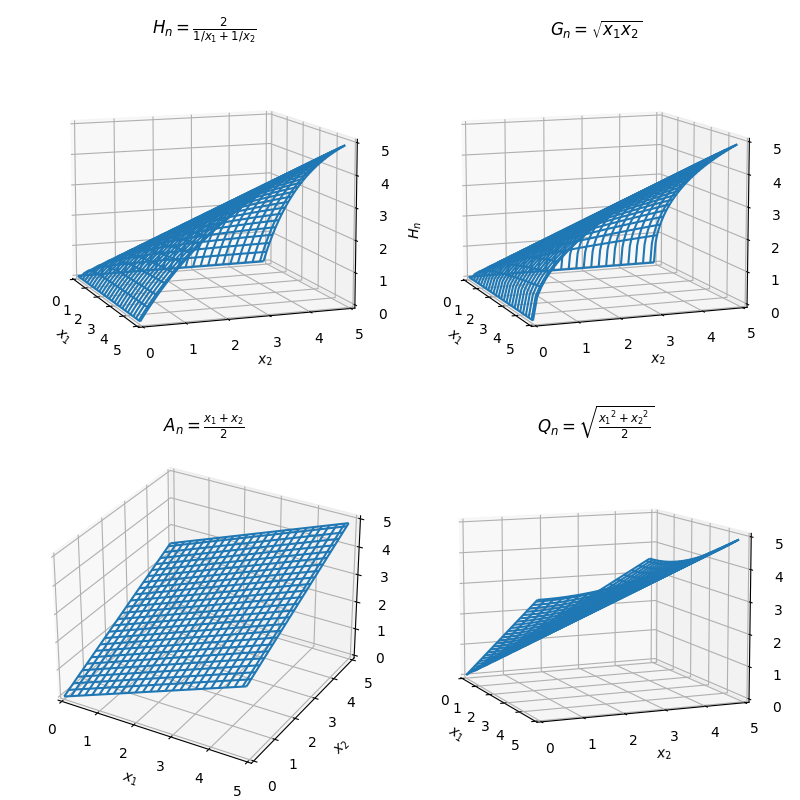
\includegraphics[height=9cm]{2.2-1.png}
\end{figure}

四类均值的图形如上,为方便作图我们只取两个变量,不难发现:
\begin{itemize}
    \item $H_n$和$G_n$弯向下,且$H_n$的下弯速度大于$G_n$;
    \item $A_n$是一个平面,必然大于$H_n$和$G_n$;
    \item $Q_n$弯向上,必然大于$A_n$;
    \item $x_1=x_2$为它们公共的交线。
\end{itemize}

\begin{theorem}[均值不等式定理]
设实数$x_1,x_2,\cdots ,x_n\in \mathbb{R} $,则四类均值有:
\[
H_n\leqslant G_n\leqslant A_n\leqslant Q_n
\]
或写成:
\[
\frac{n}{\sum_{i=i}^n{\frac{1}{x_i}}}\leqslant \sqrt[n]{x_1x_2\cdots x_n}\leqslant \frac{\sum_{i=i}^n{x_i}}{n}\leqslant \sqrt{\frac{\sum_{i=i}^n{x_{i}^{2}}}{n}}
\]
当且仅当$x_1=x_2=\cdots =x_n$时等号成立。
\end{theorem}

\begin{proof}
构造直角三角形$\bigtriangleup ABC$,如图,令$AB=\frac{x_1+x_2}{2},AC=\frac{x_1-x_2}{2}$,由勾股定理可得$BC=\sqrt{\frac{{x_1}^2+{x_2}^2}{2}}$,可见:
\[
\frac{x_1+x_2}{2}\leqslant \sqrt{\frac{{x_1}^2+{x_2}^2}{2}}
\]

\begin{figure}[h]
\centering
\begin{tikzpicture}[line join=round, scale=1]
\coordinate[label=above:{$A$}] (A) at (0,0);
\coordinate[label=above:{$C$}] (C) at (-2,0);
\coordinate[label=below:{$B$}] (B) at (0,-4);
\coordinate[label=above:{$E$}] (E) at (1.732,0);
\coordinate[label=below:{$D$}] (D) at (1.732,-3);
\coordinate[label=above:      {$\frac{x_1-x_2}{2}$}]                    (ac) at ($(A)!0.5!(C)$);
\coordinate[label=left:       {$\sqrt{\frac{x_{1}^{2}+x_{2}^{2}}{2}}$}] (bc) at ($(C)!0.5!(B)$);
\coordinate[label=above left: {$\frac{x_1+x_2}{2}$}]                    (ab) at ($(A)!0.5!(B)$);
\coordinate[label=below:      {$\sqrt{x_1x_2}$}]                        (ad) at ($(A)!0.5!(D)$);
\coordinate[label=below right:{$\frac{x_1-x_2}{2}$}]                    (bd) at ($(B)!0.5!(D)$);
\coordinate[label=right:      {$\frac{2x_1x_2}{x_1+x_2}$}]              (de) at ($(D)!0.5!(E)$);
\draw[thick] (C)--(E)--(D)--(B)--(C) (B)--(A)--(D);
\pic["$\theta $",draw,angle radius=0.5cm,angle eccentricity=1.5] {angle=B--A--D};
\pic["$\theta $",draw,angle radius=0.5cm,angle eccentricity=1.5] {angle=E--D--A};
\end{tikzpicture}
\end{figure}

再以$AB$为斜边构造直角三角形$\bigtriangleup ABD$,令$BD=AC=\frac{x_1-x_2}{2}$,由勾股定理可得$AD=\sqrt{x_1x_2}$,可见:
\[
\sqrt{x_1x_2}\leqslant \frac{x_1+x_2}{2}
\]

继续作直角三角形$\bigtriangleup ADE$,令$ED\parallel AB$,于是$\angle BAD=\angle ADE=\theta $,则有:
\begin{align*}
&\because \cos \theta =\frac{AD}{AB}=\frac{ED}{AD} \\
&\therefore ED=\frac{AD^2}{AB}=\frac{x_1x_2}{\frac{x_1+x_2}{2}}=\frac{2x_1x_2}{x_1+x_2}=\frac{2}{\frac{1}{x_1}+\frac{1}{x_2}} \\
&\therefore \frac{2}{\frac{1}{x_1}+\frac{1}{x_2}}\leqslant \sqrt{x_1x_2}
\end{align*}
\end{proof}

\begin{proof}
使用向量的方法证明
\[
\frac{x_1+x_2}{2}\leqslant \sqrt{\frac{{x_1}^2+{x_2}^2}{2}}
\]
化简如下:
\[
\frac{x_1\cdot \frac{\sqrt{2}}{2}+x_2\cdot \frac{\sqrt{2}}{2}}{\sqrt{{x_1}^2+{x_2}^2}}\leqslant 1
\]
于是就可以发现,分子是两个向量的内积,分母是向量的模,整个表达式就是两个向量夹角的余弦,于是可设$\boldsymbol{a}=\left( x_1,x_2 \right) ,\boldsymbol{b}=\left( \frac{\sqrt{2}}{2},\frac{\sqrt{2}}{2} \right) $,得到:
\[
\cos \theta =\frac{\boldsymbol{a}\cdot \boldsymbol{b}}{\left| \boldsymbol{a} \right|\left| \boldsymbol{b} \right|}=\frac{x_1\cdot \frac{\sqrt{2}}{2}+x_2\cdot \frac{\sqrt{2}}{2}}{\sqrt{{x_1}^2+{x_2}^2}}\leqslant 1
\]
\end{proof}

~

\begin{example}[综合运用4,难度:$\star $]
已知$x,y,z$都是整数,求证
\[
\left( x+y \right) \left( y+z \right) \left( z+x \right) \geqslant 8xyz
\]
\end{example}

解:

\begin{align*}
&\quad \left( x+y \right) \left( y+z \right) \left( z+x \right) \\
&=\left( xy+xz+y^2+yz \right) \left( z+x \right) \\
&=xyz+x^2y+xz^2+x^2z+y^2z+y^2x+yz^2+xyz
\end{align*}
观察分析:
\begin{align*}
&x^2y+yz^2\geqslant 2y\sqrt{x^2z^2}=2xyz \\
&xz^2+y^2x\geqslant 2x\sqrt{z^2y^2}=2xyz \\
&x^2z+y^2z\geqslant 2z\sqrt{x^2y^2}=2xyz
\end{align*}
略,证毕。

\begin{tcolorbox}
本题只需尝试将左边展开即可发现方法。
\end{tcolorbox}

~

\begin{example}[拓广探索7,难度:$\star \star $]
一家商店使用一架两臂不等长的天平秤黄金,一位顾客到商店购买10g黄金,售货员先将5g的砝码放在天平左盘中,取出一些黄金放在天平右盘中使天平平衡;再将5g的砝码放在天平的右盘中,再取出一些黄金放在天平左盘中使天平平衡;最后将两次称得的黄金交给顾客。你认为顾客购得的黄金是小于10g,等于10g,还是大于10g?为什么?
\end{example}

解:

这个问题较为复杂,我们可以先尝试用一些数学式子描述该问题。假设天平左右两个臂的臂长分别为$l_L,l_R$,则根据力矩相等易得两次称重黄金的数学表示为:
\begin{align*}
&5\cdot l_L=A\cdot l_R \\
&B\cdot l_L=5\cdot l_R
\end{align*}
稍稍化简得:
\begin{align*}
&A=5\cdot \frac{l_L}{l_R} \\
&B=5\cdot \frac{l_R}{l_L}
\end{align*}
易得:
\[
A+B\geqslant 2\sqrt{5\cdot \frac{l_L}{l_R}\cdot 5\cdot \frac{l_R}{l_L}}=10
\]

\begin{tcolorbox}
本题关键在于获得$A,B$的表达式,一旦获得了,不难发现其互为倒数的关系,也就能自然想到基本不等式了。
\end{tcolorbox}

~

\begin{example}[拓广探索8,难度:$\star \star $]
设矩形$ABCD$($AB>AD$)的周长为24cm,把$\bigtriangleup ABC$沿$AC$向$\bigtriangleup ADC$折叠,$AB$折过去后交$DC$于点$P$。
设$AB=x\mathrm{cm}$,求$\bigtriangleup ADP$的最大面积及相应$x$的值。
\end{example}

\begin{figure}[h]
\centering
\begin{tikzpicture}[line join=round, scale=0.75]
\coordinate[label=above left: {$A$}]  (A)  at (-2.5,1);
\coordinate[label=above right:{$B$}]  (B)  at (2.5,1);
\coordinate[label=below right:{$C$}]  (C)  at (2.5,-1);
\coordinate[label=below left: {$D$}]  (D)  at (-2.5,-1);
\draw[thick] (D)--(A)--(B)--(C) (A)--(C);
\coordinate                     (tb) at ($(A)!(B)!(C)$);
\coordinate[label=below:{$B'$}] (B') at ($(B)!2.0!(tb)$);
\draw[thick,name path=l1] (D)--(C);
\draw[thick,blue,name path=l2] (A)--(B');
\path [name intersections={of=l1 and l2}] coordinate[label=below left:$P$] (P) at (intersection-1);
\draw[thick,blue] (B')--(C);
\coordinate                           (tp) at ($(A)!(P)!(C)$);
\coordinate[label=above right:{$P'$}] (P') at ($(P)!2.0!(tp)$);
\draw[thick,dashed,red] (P)--(P')--(C);
\coordinate[label=above:{$x$}]    (x)  at ($(A)!0.5!(B)$);
\coordinate[label=left: {$12-x$}] (x') at ($(A)!0.5!(D)$);
\coordinate[label=below:{$y$}]    (y)  at ($(D)!0.5!(P)$);
\end{tikzpicture}
\end{figure}

解:

令$DP$长$y$,则$\bigtriangleup ADP$的面积为:
\[
S_{\bigtriangleup ADP}=\frac{1}{2}\left( 12-x \right) y
\]
不难证明$\bigtriangleup ADP,\bigtriangleup CB'P$均为直角三角形,且全等,于是
\begin{align*}
&\because PC=PA=\sqrt{\left( 12-x \right) ^2+y^2} \\
&\therefore x=\sqrt{\left( 12-x \right) ^2+y^2}+y \\
&\therefore y=\frac{12x-72}{x}
\end{align*}
带入面积消去$y$,得:
\begin{align*}
S_{\bigtriangleup ADP}&=\frac{1}{2}\left( 12-x \right) y=\frac{1}{2}\left( 12-x \right) \frac{12x-72}{x} \\
&=6\cdot \frac{-x^2+18x-72}{x} \\
&=6\cdot \left( -x-\frac{72}{x}+18 \right)
\end{align*}
其中,$x+\frac{72}{x}\geqslant 2\sqrt{72}=12\sqrt{2}$,当且仅当$x=\frac{72}{x},x=\sqrt{72}$时等号成立,于是:
\[
S_{\bigtriangleup ADP}\leqslant 6\cdot \left( 18-12\sqrt{2} \right)
\]

\begin{tcolorbox}
本题的关键在于获得$S_{\bigtriangleup ADP}$的表达式和$x,y$的约束关系。一旦获得了,接下去就是化简和基本不等式。
\end{tcolorbox}

\begin{tcolorbox}
高中阶段的求解最值问题,最终都会转化为求解
\[
\left( Ax \right) +\left( \frac{B}{x} \right) \quad \text{或} \quad \left( Ax \right) \cdot \left( \frac{B}{x} \right)
\]
的最值问题,也即基本不等式。关键在于理解问题和观察图形,将实际问题或几何图形建模成代数问题。上面两题很有典型性,一题是实际应用题,另一题是几何题。结合上一章的说到的数学范式,认真思考上面两题,总结你的解题范式,XML。
\end{tcolorbox}






\newpage
\section{二次函数与一元二次方程、不等式}

本节要点:
\begin{itemize}
    \item 从基本不等式深刻理解二次函数的最值。
\end{itemize}

~

虽然二次函数的标准形式为$y=ax^2+bx+c$,但以下方式更能说明二次函数:
\[
y=a\left( x+b \right) ^2+c
\]
\begin{itemize}
    \item 首先,通过$a$变换开口大小和方向,$a$越小开口越宽大,$a>0$开口向上;
    \item 然后,通过$b$进行沿{\it x}轴的平移,$b>0$左移;
    \item 最后,通过$c$进行沿{\it y}轴的平移,$c>0$上移。
\end{itemize}

\begin{figure}[h]
\centering
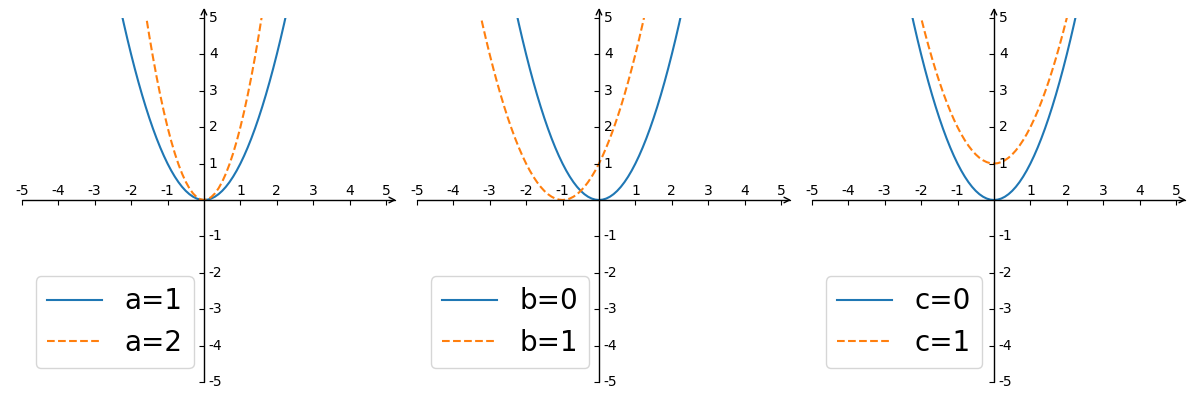
\includegraphics[height=4cm]{2.3-1.png}
\end{figure}

二次函数和基本不等式也可以相互推导。设某个变量$y$由$x,z$乘积决定,而$x,z$有关系$x+z=c$,其中 $c$为常数,于是:
\[
\begin{cases}
	y=x\cdot z\\
	x+z=c\\
\end{cases}\Rightarrow y=x\cdot \left( c-x \right)
\]
由基本不等式可得:
\[
y=x\cdot \left( c-x \right) \leqslant \left[ \frac{x+\left( c-x \right)}{2} \right] ^2=\frac{c^2}{4}
\]
用二次函数的方法:
\[
y=-x^2+cx
\]
当且仅当$x=\frac{c}{2}$时,$y$取最大值$y_{\max}=\frac{c^2}{4}$。

\begin{tcolorbox}
当两个变量的和为常量时,它们的积有最大值,这点从基本不等式和二次函数都能得到一样的结果。
\end{tcolorbox}

\begin{tcolorbox}
工程中,我们通常为最值构造一个二次函数$y=f\left( x_1,x_2 \right) $,用$ax_1+bx_2=c$作为两个变量的约束条件,得到一个二次函数,最终可求解最值。
\end{tcolorbox}

~

\begin{example}[综合运用4,难度:$\star $]
一名同学以初速度$v_0=12\mathrm{m}/\mathrm{s}$竖直向上抛一排球,排球能够在抛出点2m以上大的位置最多停留多长时间(精确到0.01s)?
\end{example}

\begin{figure}[h]
\centering
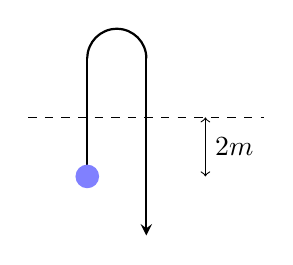
\begin{tikzpicture}[line join=round, scale=0.75]
\draw[thick] (0,0)--(0,2);
\draw[thick] (1,2) arc [start angle=0,end angle=180,radius=0.5cm];
\draw[thick,-stealth] (1,2)--(1,-1);
\fill[blue!50!white] (0,0) circle (2mm);
\draw[dashed] (-1,1)--(3,1);
\draw[<->] (2,1)--(2,0);
\coordinate[label=right:{$2m$}] (t) at (2,0.5);
\end{tikzpicture}
\end{figure}

解:

排球距抛出点高度和时间的关系如下:
\[
h=v_0t-\frac{1}{2}gt^2
\]
带入$v_0=12\mathrm{m}/\mathrm{s},g=10\mathrm{m}/\mathrm{s}^2,h\geqslant 2\mathrm{m}$得:
\[
12t-5t^2\geqslant 2
\]
令$5t^2-12t+2=0$,解得$t_{1,2}=\frac{12\pm \sqrt{12^2-4\cdot 5\cdot 2}}{2\cdot 5}=2.220 \,\, \mathrm{or} \,\, 0.180$,于是停留时间为$t=2.220-0.180=2.04\mathrm{s}$。

\begin{tcolorbox}
本题看似难,其实一点不难,物理问题已经转化为数学问题,剩下的就是体力活。
\end{tcolorbox}






\newpage
\section{扩展知识:\texorpdfstring{$y=x+\frac{1}{x}$}{y=x+1/x}的图形}

本节我们绘制
\[
y=ax+\frac{b}{x}
\]
的图形,以加深对基本不等式的理解。

~

由于函数是奇函数,且$x\ne 0$,所以我们只绘制$x>0$部分,先从最基本的开始,如下函数:
\[
y=x+\frac{1}{x} \qquad x>0
\]
图形如下,不难发现:
\begin{itemize}
    \item 图形由两部分组成,左边是$\frac{1}{x}$主导,右边是$x$主导;
    \item $y$先减小后增大,当$x=1$时取最小值2;
    \item $x=0$和$y=x$是函数的两条渐近线。
\end{itemize}

\begin{figure}[h]
\centering
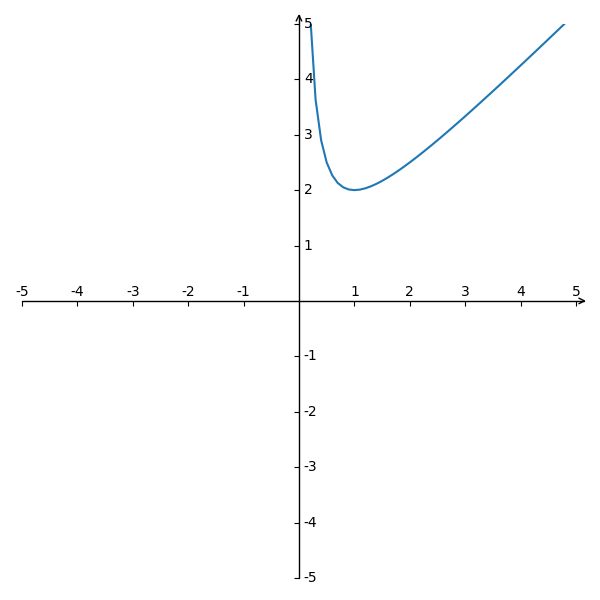
\includegraphics[height=6cm]{2.4-1.png}
\end{figure}

~

若我们调整$a$
\begin{align*}
&y=0.5x+\frac{1}{x} \\
&y=x+\frac{1}{x} \\
&y=2x+\frac{1}{x}
\end{align*}
则函数图形如下。

\begin{figure}[ht]
\centering
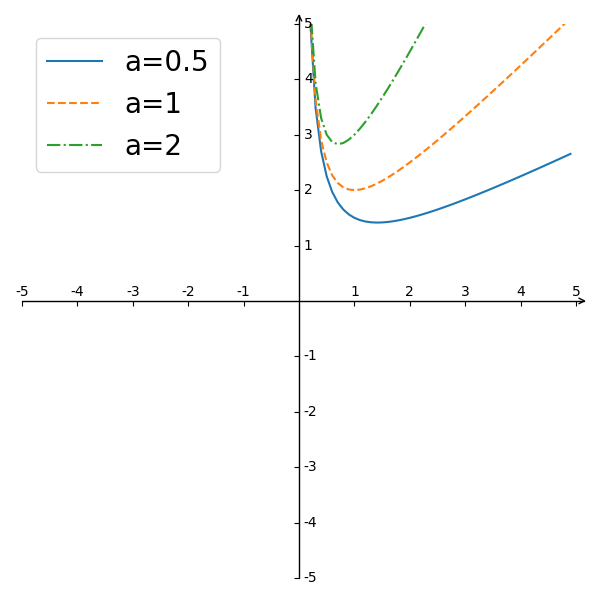
\includegraphics[height=6cm]{2.4-2.png}
\end{figure}

~

若我们调整$b$
\begin{align*}
&y=x+\frac{0.5}{x} \\
&y=x+\frac{1}{x} \\
&y=x+\frac{2}{x}
\end{align*}
则函数图形如下。

\begin{figure}[h]
\centering
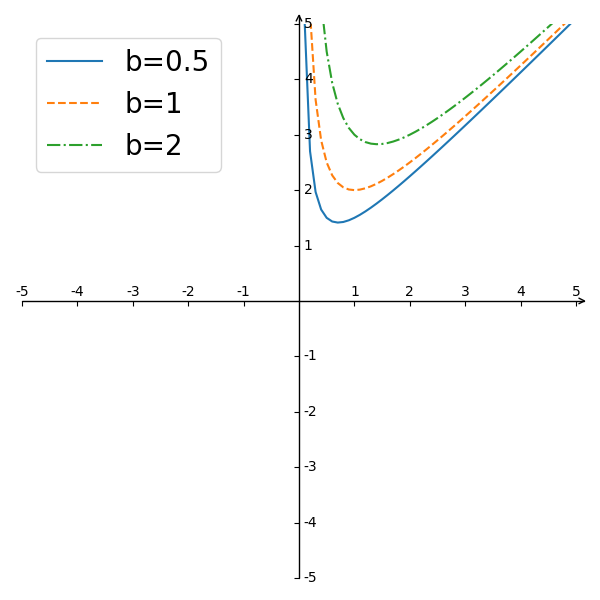
\includegraphics[height=6cm]{2.4-3.png}
\end{figure}

不难发现:
\begin{itemize}
    \item 调节$a$,影响的是$x$部分,图象上反映在右侧变化较大;
    \item 调节$b$,影响的是$1/x$部分,图象上反映在左侧变化较大;
    \item 无论调节$a$还是$b$,最值都会发生变化。
\end{itemize}






\newpage
\section{本章小结}

本章讨论了不等式,特别讨论了基本不等式和二次函数的最值。

特别要注意四类均值及其关系:
\[
\frac{n}{\sum_{i=i}^n{\frac{1}{x_i}}}\leqslant \sqrt[n]{x_1x_2\cdots x_n}\leqslant \frac{\sum_{i=i}^n{x_i}}{n}\leqslant \sqrt{\frac{\sum_{i=i}^n{x_{i}^{2}}}{n}}
\]
即:
\[
\text{调和}\leqslant \text{几何}\leqslant \text{算数}\leqslant \text{平方}
\]

其次要将基本不等式和二次函数的最值两者融会贯通,通过基本不等式分析二次函数最值的由来。

~

\begin{example}[综合运用5,难度:$\star $]
若$a,b>0$,且$ab=a+b+3$,求$ab$的取值范围。
\end{example}

解一:

题意为求函数$y=ab$的取值范围,且$a,b$有约束$ab=a+b+3$。将约束化简得:
\[
a=\frac{b+3}{b-1} \qquad b>1
\]
带入函数得到:
\[
y=ab=b\cdot \frac{b+3}{b-1} \qquad b>1
\]
不是很明显,但有$x\cdot \frac{1}{x}$的形式,化简该函数:
\begin{align*}
y=b\cdot \frac{b-1+4}{b-1}=\frac{4b}{b-1}+b=\frac{4b-4+4}{b-1}+b=\frac{4}{b-1}+\left( b-1 \right) +5
\end{align*}
易得$\left( b-1 \right) ^2=4$即$b=3$时,$y$有最小值$y_{\min}=9$,函数图象如下。
\begin{figure}[h]
\centering
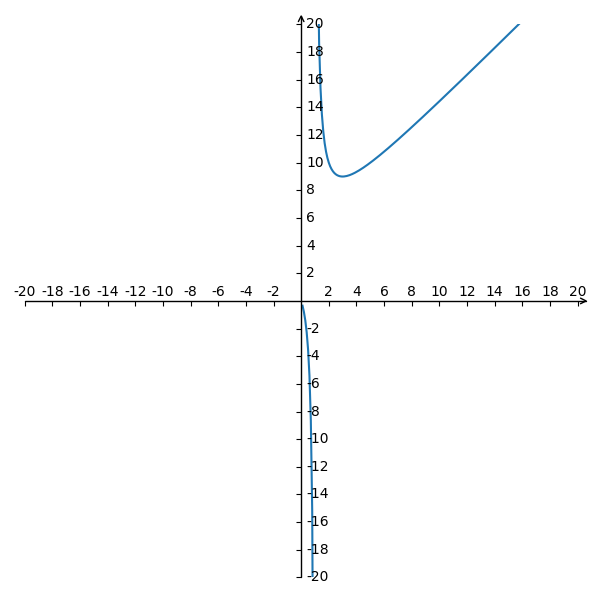
\includegraphics[height=5cm]{2.5-1.png}
\end{figure}

这里,我们将$b\in \left( 0,1 \right) $部分绘制出来,但是由于$a>$的限制,实际$b$的取值范围为$\left( 1,+\infty \right) $。

解二:

观察约束条件和要求的取值函数,$a,b$对称,所以可以直接考察约束条件:
\[
ab=a+b+3\geqslant 2\sqrt{ab}+3
\]
当且仅当$a=b$时成立。于是,可令$y=\sqrt{ab}$,替换得到:
\[
y^2\geqslant y+3 \qquad y>0
\]
易得$y\geqslant 3$,所以当$a=b$时,$ab$取得最小值9。

\begin{tcolorbox}
解一是正经方法,采用了一贯的套路,表达式+约束关系,化简,用基本不等式求解。解二不正经,需要多练,提高洞察力。
\end{tcolorbox}









